\documentclass[10pt,a4paper,titlepage,parskip]{scrartcl}
\usepackage[utf8]{inputenc}
\usepackage{pdfpages}
\usepackage[english]{babel}
\renewcommand\familydefault{\sfdefault}
\usepackage{color}
\usepackage{etoolbox}
\usepackage{lastpage}
\usepackage{hyperref}
\usepackage{framed}
\usepackage{subcaption}
\usepackage{enumerate}
\usepackage{amssymb}

% adjust the page margins
\usepackage[left=2.5cm,right=2.5cm,top=2.5cm,bottom=3.0cm]{geometry}

\usepackage{fancyhdr}
\pagestyle{fancy}

\definecolor{myBlue}{rgb}{0.2,0.4,0.65}
\definecolor{ufzgray1}{RGB}{81,81,81}
\definecolor{ufzgray2}{RGB}{156,156,156}
\definecolor{ufzgray3}{RGB}{185,185,185}

\patchcmd{\headrule}{\hrule}{\color{myBlue}\hrule}{}{}
\patchcmd{\footrule}{\hrule}{\color{myBlue}\hrule}{}{}

% dots after section numbers
\renewcommand{\thesection}{\arabic{section}.}
\renewcommand{\thesubsection}{\arabic{section}.\arabic{subsection}.}

% make an entire region tt font
\newenvironment{ttfont}{\fontfamily{\ttdefault}\selectfont}{\par}

% My style
\usepackage{xcolor}
\definecolor{jmcolor}{RGB}{255,127,0}
\newcommand{\jm}[1]{\textcolor{jmcolor}{#1}}
\newcommand{\jmout}[1]{\textcolor{jmcolor}{\sout{#1}}}
\newcommand{\GRAU}[1]{\textcolor{ufzgray2}{#1}}

%\newcommand{\footrulecolor}{myBlue}
\rhead{}
\lhead{}
\chead{\textcolor{myBlue}{\footnotesize Project Documentation ``Improving characterization of flood-producing precipitation events in HFE database''}}
\lfoot{\textcolor{myBlue}{\footnotesize Telephone: +1 (226) 505-5600}}
\cfoot{\textcolor{myBlue}{\footnotesize e-mail: juliane.mai@uwaterloo.ca}}
\rfoot{\textcolor{myBlue}{\footnotesize Page \thepage \ of \pageref{LastPage}}}
\renewcommand{\footrulewidth}{0.4pt} 

% Hurenkinder und Schusterjungen verhindern
\clubpenalty10000
\widowpenalty10000
\displaywidowpenalty=10000

\includepdfset{pages=-}

% colored lines
\makeatletter
\let\old@rule\@rule
\def\@rule[#1]#2#3{\textcolor{rulecolor}{\old@rule[#1]{#2}{#3}}}
\makeatother

% fixed width columns in table
\usepackage{array}
\newcolumntype{L}[1]{>{\raggedright\let\newline\\\arraybackslash\hspace{0pt}}p{#1}}
\newcolumntype{C}[1]{>{\centering\let\newline\\\arraybackslash\hspace{0pt}}p{#1}}
\newcolumntype{R}[1]{>{\raggedleft\let\newline\\\arraybackslash\hspace{0pt}}p{#1}}

%\linespread{1.5}

\begin{document}  
	
	\vspace*{-1cm}
	\pagestyle{fancy}
	
	\begin{center}
		Juliane Mai, Ph.D.\\
		Technical Consulting\\[4pt]
		405-460A Belmont Ave W., \\
		Kitchener, ON, N2M 0A9, Canada\\[10pt]
		{\definecolor{rulecolor}{named}{myBlue}\rule{\linewidth}{0.4pt}}
	\end{center}
	\begin{center}
		\textcolor{myBlue}{{\Large --~Comparison of CaSPAr and GeoMet data~--}}\\[20pt]
	\end{center}
	A comparison of a selected number of 23 floods (single-point from ``historical\_flood.json'') that all occurred in 2017 such that data from RDRS\_v2.1 as well as RDPA-6h are available on CaSPAr and GeoMet, respectively.
	
	The data have been downloaded and analyzed using the same approach to identify the main precipitation event (highlighted blue bars). The sum of precipitation identified and then considered as the main precipitation amount is reported in the label at the bottom of each figure. Each page contains the results for one event; one plot using data from CaSPAr (panel a) and one plot for data from GeoMet (panel b).
	
	Gaps in plots only occur for GeoMet (panel b) when the data are not available.
	
	\vfill
	Version: 1.0\\
	Date: Sep 21, 2022\\
	
	
\pagebreak

\begin{figure}[h]
	\begin{subfigure}[a]{1.0\textwidth}
		\centering
		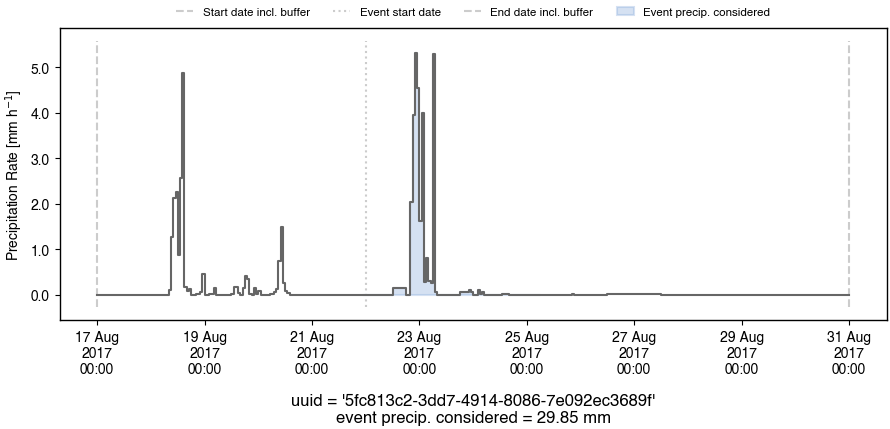
\includegraphics[width=\linewidth]{figures/compare_Geomet_CaSPAr/interpolated_at_stations_occurrence_794_identified-timesteps_RDRS_v2.1.png}
		\caption{Flood occurrence analyzed using data from CaSPAr NetCDF data (RDRS\_v2.1; 1hr accumulations)}
	\end{subfigure}
	%\vspace*{0.05\textwidth}
	\par\bigskip\bigskip
	\begin{subfigure}[b]{1.0\textwidth}
		\centering
		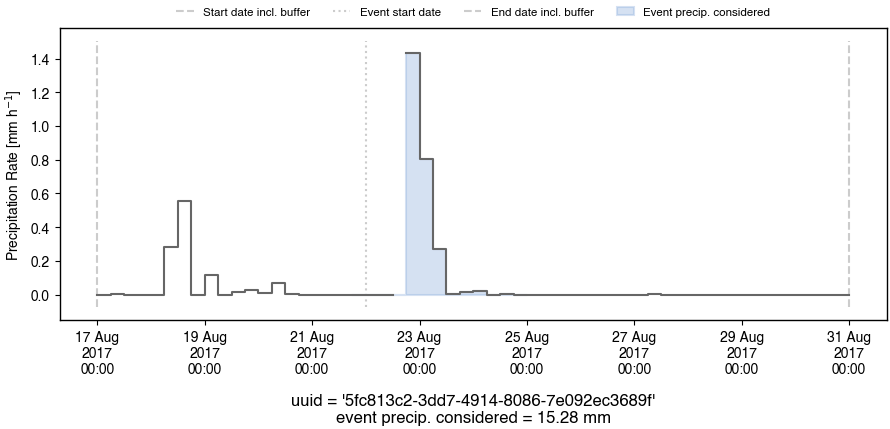
\includegraphics[width=\linewidth]{figures/compare_Geomet_CaSPAr/interpolated_at_stations_occurrence_794_identified-timesteps_rdpa:10km:6f.png}
		\caption{Flood occurrence analyzed using data from GeoMet GRIB2 data (RDPA; 6hr accumulations)}
	\end{subfigure}
	\par\bigskip\bigskip
	\caption{Flood occurrence in 2017 from HFE database (historical\_flood.json) with UUID ``5fc813c2-3dd7-4914-8086-7e092ec3689f''}
\end{figure}
\pagebreak

\begin{figure}[h]
	\begin{subfigure}[a]{1.0\textwidth}
		\centering
		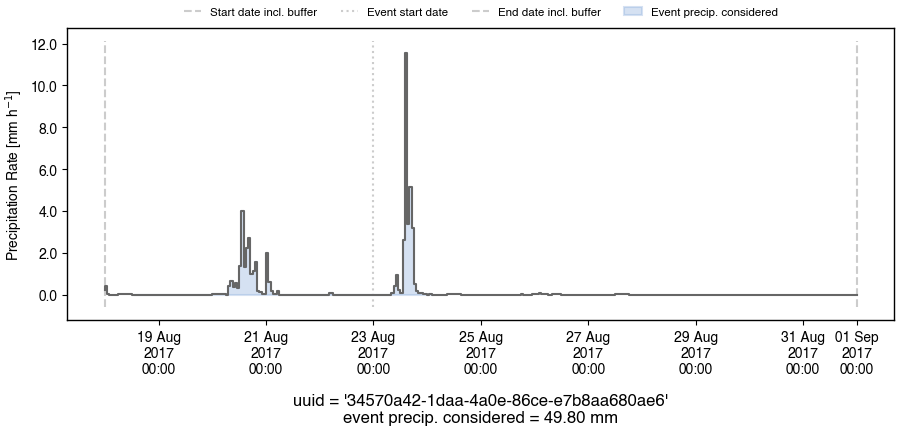
\includegraphics[width=\linewidth]{figures/compare_Geomet_CaSPAr/interpolated_at_stations_occurrence_883_identified-timesteps_RDRS_v2.1.png}
		\caption{Flood occurrence analyzed using data from CaSPAr NetCDF data (RDRS\_v2.1; 1hr accumulations)}
	\end{subfigure}
	%\vspace*{0.05\textwidth}
	\par\bigskip\bigskip
	\begin{subfigure}[b]{1.0\textwidth}
		\centering
		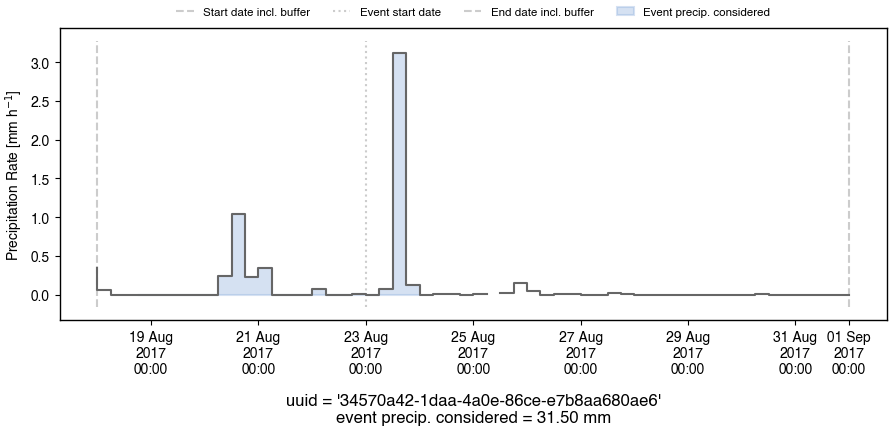
\includegraphics[width=\linewidth]{figures/compare_Geomet_CaSPAr/interpolated_at_stations_occurrence_883_identified-timesteps_rdpa:10km:6f.png}
		\caption{Flood occurrence analyzed using data from GeoMet GRIB2 data (RDPA; 6hr accumulations)}
	\end{subfigure}
	\par\bigskip\bigskip
	\caption{Flood occurrence in 2017 from HFE database (historical\_flood.json) with UUID ``34570a42-1daa-4a0e-86ce-e7b8aa680ae6''}
\end{figure}
\pagebreak

\begin{figure}[h]
	\begin{subfigure}[a]{1.0\textwidth}
		\centering
		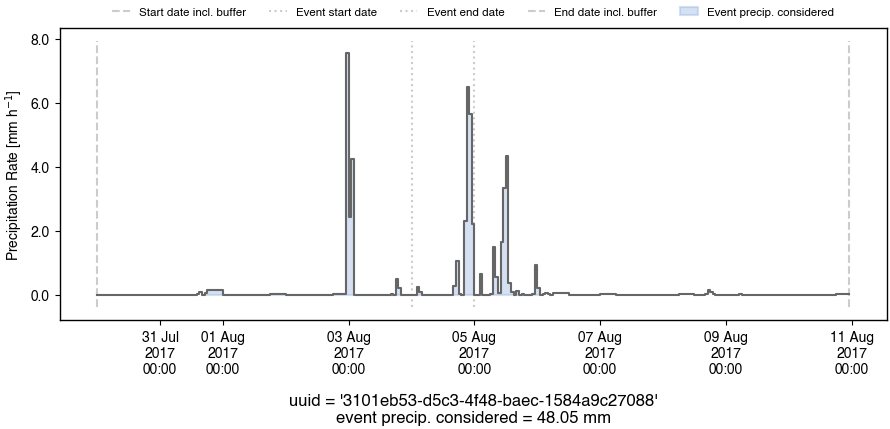
\includegraphics[width=\linewidth]{figures/compare_Geomet_CaSPAr/interpolated_at_stations_occurrence_932_identified-timesteps_RDRS_v2.1.png}
		\caption{Flood occurrence analyzed using data from CaSPAr NetCDF data (RDRS\_v2.1; 1hr accumulations)}
	\end{subfigure}
	%\vspace*{0.05\textwidth}
	\par\bigskip\bigskip
	\begin{subfigure}[b]{1.0\textwidth}
		\centering
		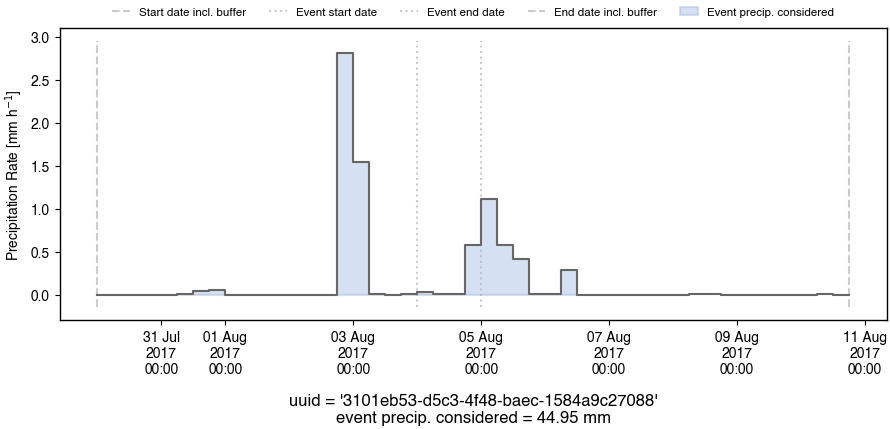
\includegraphics[width=\linewidth]{figures/compare_Geomet_CaSPAr/interpolated_at_stations_occurrence_932_identified-timesteps_rdpa:10km:6f.png}
		\caption{Flood occurrence analyzed using data from GeoMet GRIB2 data (RDPA; 6hr accumulations)}
	\end{subfigure}
	\par\bigskip\bigskip
	\caption{Flood occurrence in 2017 from HFE database (historical\_flood.json) with UUID ``3101eb53-d5c3-4f48-baec-1584a9c27088''}
\end{figure}
\pagebreak

\begin{figure}[h]
	\begin{subfigure}[a]{1.0\textwidth}
		\centering
		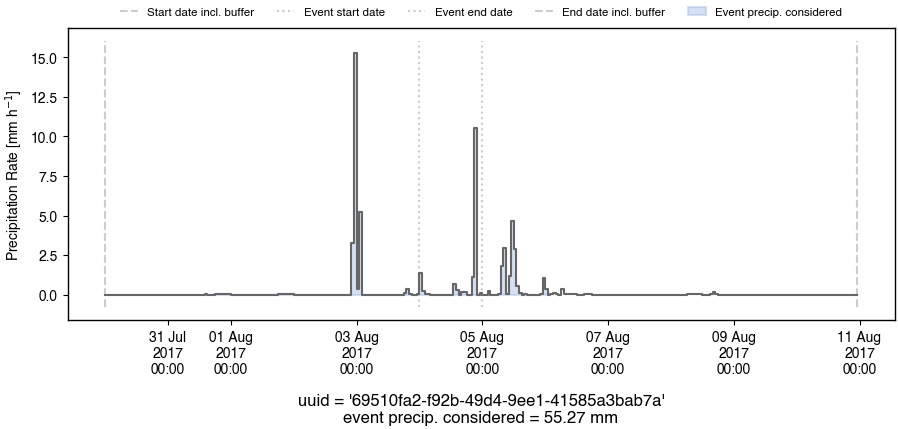
\includegraphics[width=\linewidth]{figures/compare_Geomet_CaSPAr/interpolated_at_stations_occurrence_936_identified-timesteps_RDRS_v2.1.png}
		\caption{Flood occurrence analyzed using data from CaSPAr NetCDF data (RDRS\_v2.1; 1hr accumulations)}
	\end{subfigure}
	%\vspace*{0.05\textwidth}
	\par\bigskip\bigskip
	\begin{subfigure}[b]{1.0\textwidth}
		\centering
		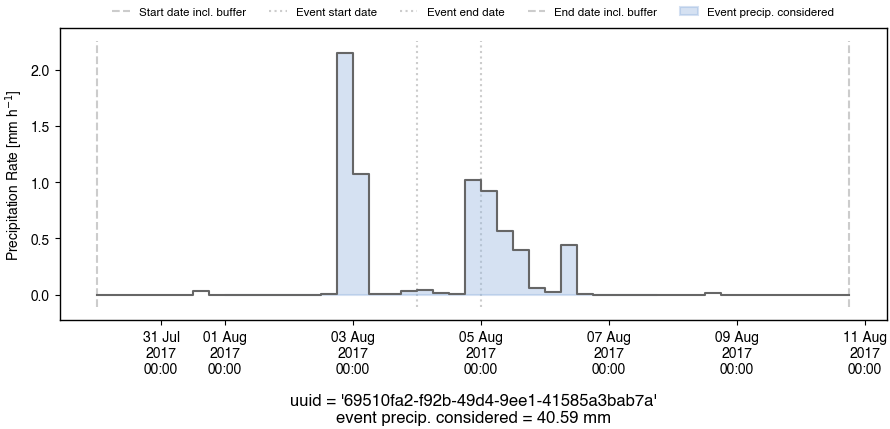
\includegraphics[width=\linewidth]{figures/compare_Geomet_CaSPAr/interpolated_at_stations_occurrence_936_identified-timesteps_rdpa:10km:6f.png}
		\caption{Flood occurrence analyzed using data from GeoMet GRIB2 data (RDPA; 6hr accumulations)}
	\end{subfigure}
	\par\bigskip\bigskip
	\caption{Flood occurrence in 2017 from HFE database (historical\_flood.json) with UUID ``69510fa2-f92b-49d4-9ee1-41585a3bab7a''}
\end{figure}
\pagebreak

\begin{figure}[h]
	\begin{subfigure}[a]{1.0\textwidth}
		\centering
		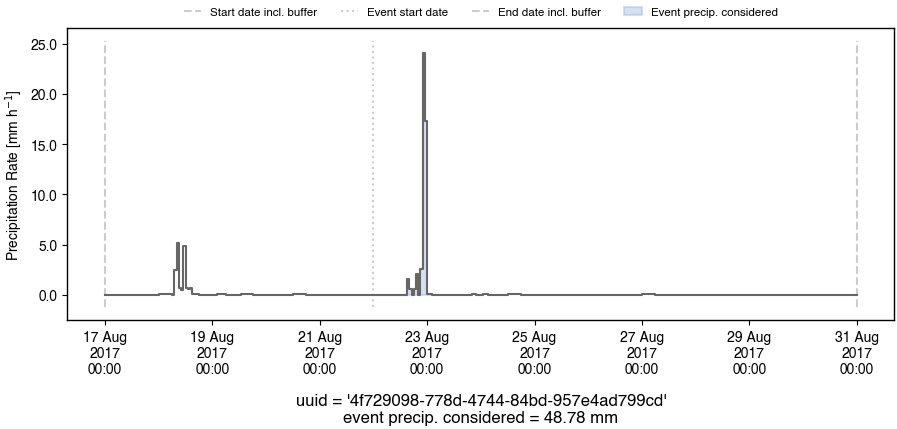
\includegraphics[width=\linewidth]{figures/compare_Geomet_CaSPAr/interpolated_at_stations_occurrence_963_identified-timesteps_RDRS_v2.1.png}
		\caption{Flood occurrence analyzed using data from CaSPAr NetCDF data (RDRS\_v2.1; 1hr accumulations)}
	\end{subfigure}
	%\vspace*{0.05\textwidth}
	\par\bigskip\bigskip
	\begin{subfigure}[b]{1.0\textwidth}
		\centering
		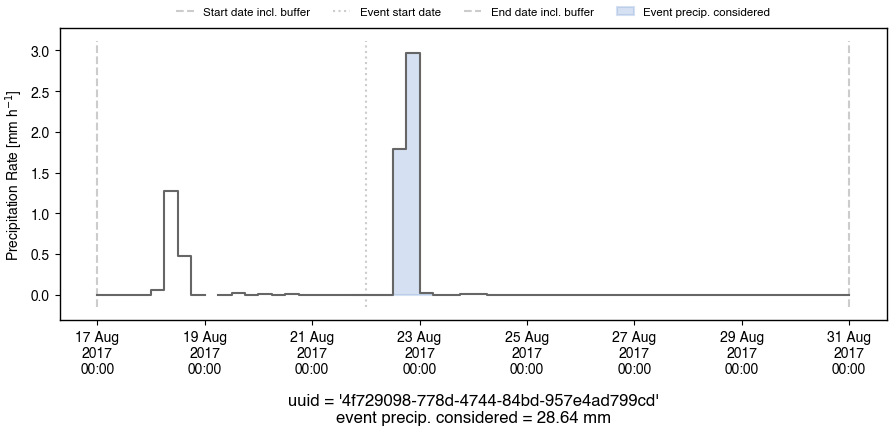
\includegraphics[width=\linewidth]{figures/compare_Geomet_CaSPAr/interpolated_at_stations_occurrence_963_identified-timesteps_rdpa:10km:6f.png}
		\caption{Flood occurrence analyzed using data from GeoMet GRIB2 data (RDPA; 6hr accumulations)}
	\end{subfigure}
	\par\bigskip\bigskip
	\caption{Flood occurrence in 2017 from HFE database (historical\_flood.json) with UUID ``4f729098-778d-4744-84bd-957e4ad799cd''}
\end{figure}
\pagebreak

\begin{figure}[h]
	\begin{subfigure}[a]{1.0\textwidth}
		\centering
		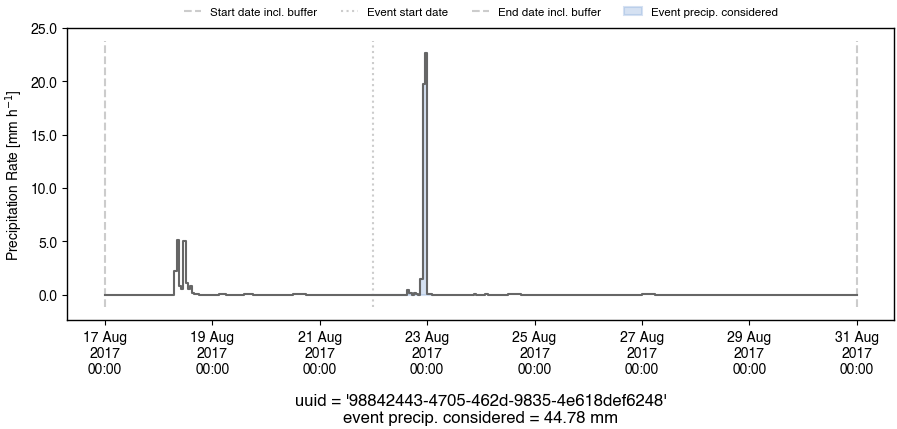
\includegraphics[width=\linewidth]{figures/compare_Geomet_CaSPAr/interpolated_at_stations_occurrence_965_identified-timesteps_RDRS_v2.1.png}
		\caption{Flood occurrence analyzed using data from CaSPAr NetCDF data (RDRS\_v2.1; 1hr accumulations)}
	\end{subfigure}
	%\vspace*{0.05\textwidth}
	\par\bigskip\bigskip
	\begin{subfigure}[b]{1.0\textwidth}
		\centering
		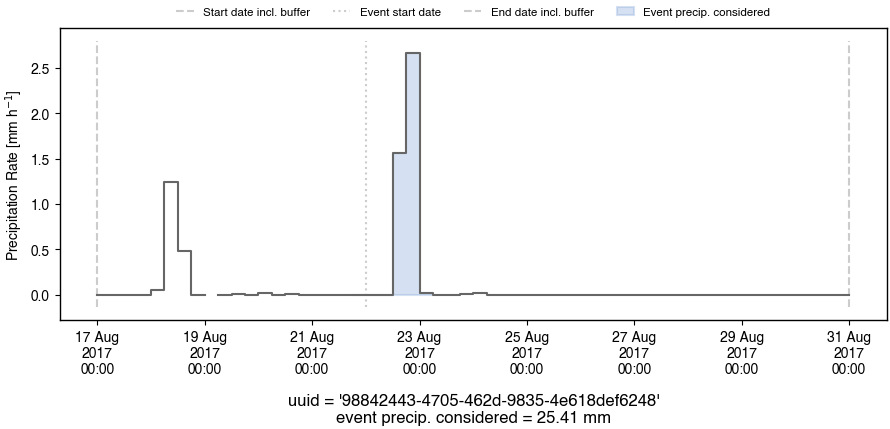
\includegraphics[width=\linewidth]{figures/compare_Geomet_CaSPAr/interpolated_at_stations_occurrence_965_identified-timesteps_rdpa:10km:6f.png}
		\caption{Flood occurrence analyzed using data from GeoMet GRIB2 data (RDPA; 6hr accumulations)}
	\end{subfigure}
	\par\bigskip\bigskip
	\caption{Flood occurrence in 2017 from HFE database (historical\_flood.json) with UUID ``98842443-4705-462d-9835-4e618def6248''}
\end{figure}
\pagebreak

\begin{figure}[h]
	\begin{subfigure}[a]{1.0\textwidth}
		\centering
		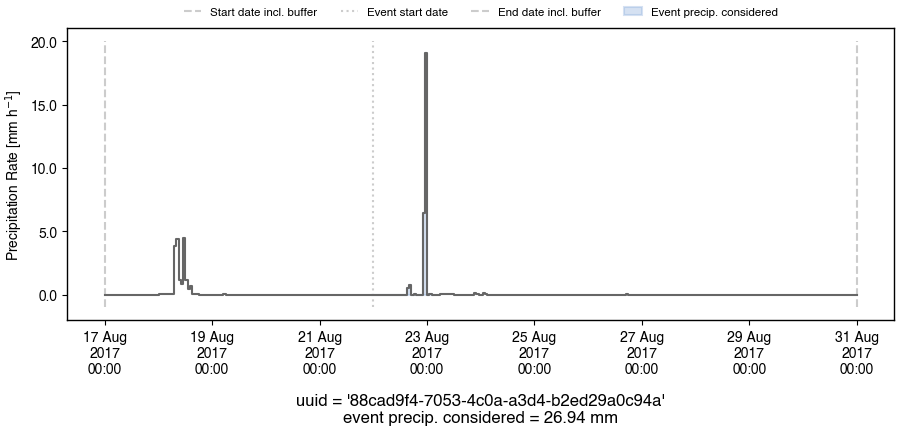
\includegraphics[width=\linewidth]{figures/compare_Geomet_CaSPAr/interpolated_at_stations_occurrence_1008_identified-timesteps_RDRS_v2.1.png}
		\caption{Flood occurrence analyzed using data from CaSPAr NetCDF data (RDRS\_v2.1; 1hr accumulations)}
	\end{subfigure}
	%\vspace*{0.05\textwidth}
	\par\bigskip\bigskip
	\begin{subfigure}[b]{1.0\textwidth}
		\centering
		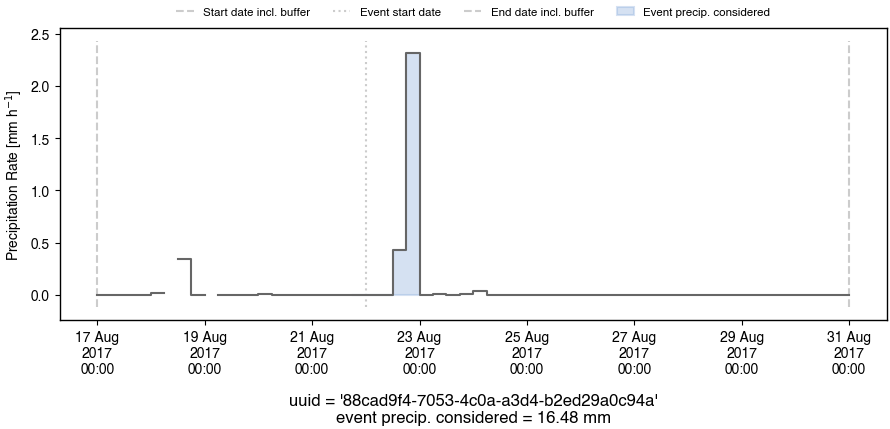
\includegraphics[width=\linewidth]{figures/compare_Geomet_CaSPAr/interpolated_at_stations_occurrence_1008_identified-timesteps_rdpa:10km:6f.png}
		\caption{Flood occurrence analyzed using data from GeoMet GRIB2 data (RDPA; 6hr accumulations)}
	\end{subfigure}
	\par\bigskip\bigskip
	\caption{Flood occurrence in 2017 from HFE database (historical\_flood.json) with UUID ``88cad9f4-7053-4c0a-a3d4-b2ed29a0c94a''}
\end{figure}
\pagebreak

\begin{figure}[h]
	\begin{subfigure}[a]{1.0\textwidth}
		\centering
		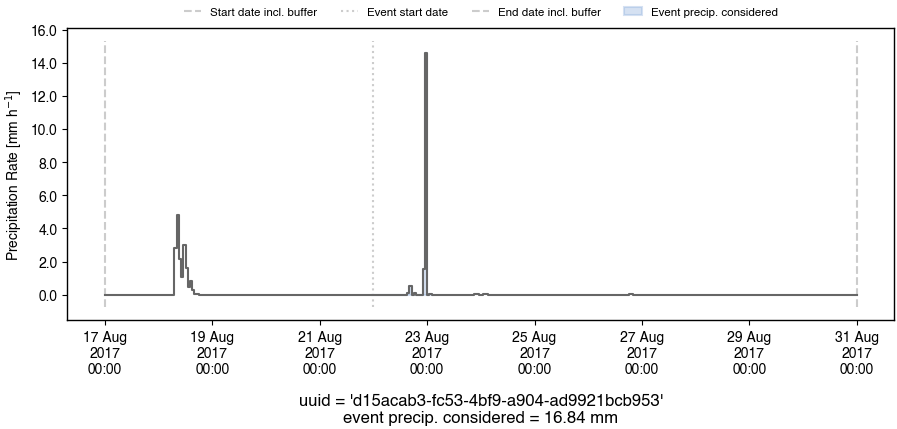
\includegraphics[width=\linewidth]{figures/compare_Geomet_CaSPAr/interpolated_at_stations_occurrence_1009_identified-timesteps_RDRS_v2.1.png}
		\caption{Flood occurrence analyzed using data from CaSPAr NetCDF data (RDRS\_v2.1; 1hr accumulations)}
	\end{subfigure}
	%\vspace*{0.05\textwidth}
	\par\bigskip\bigskip
	\begin{subfigure}[b]{1.0\textwidth}
		\centering
		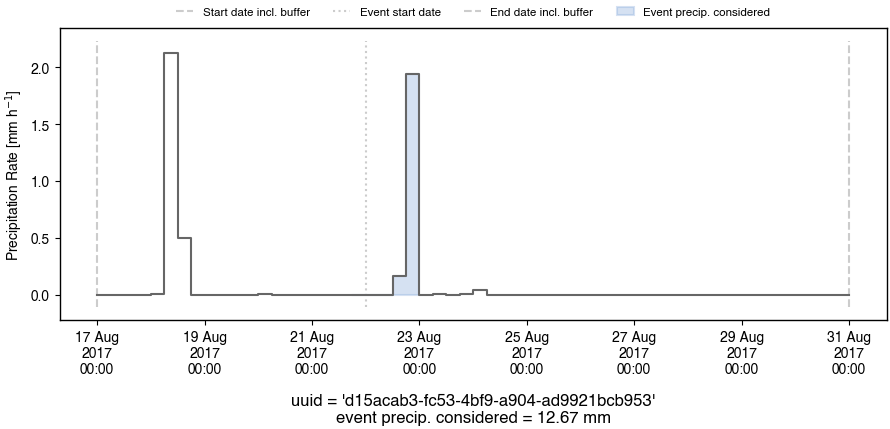
\includegraphics[width=\linewidth]{figures/compare_Geomet_CaSPAr/interpolated_at_stations_occurrence_1009_identified-timesteps_rdpa:10km:6f.png}
		\caption{Flood occurrence analyzed using data from GeoMet GRIB2 data (RDPA; 6hr accumulations)}
	\end{subfigure}
	\par\bigskip\bigskip
	\caption{Flood occurrence in 2017 from HFE database (historical\_flood.json) with UUID ``d15acab3-fc53-4bf9-a904-ad9921bcb953''}
\end{figure}
\pagebreak

\begin{figure}[h]
	\begin{subfigure}[a]{1.0\textwidth}
		\centering
		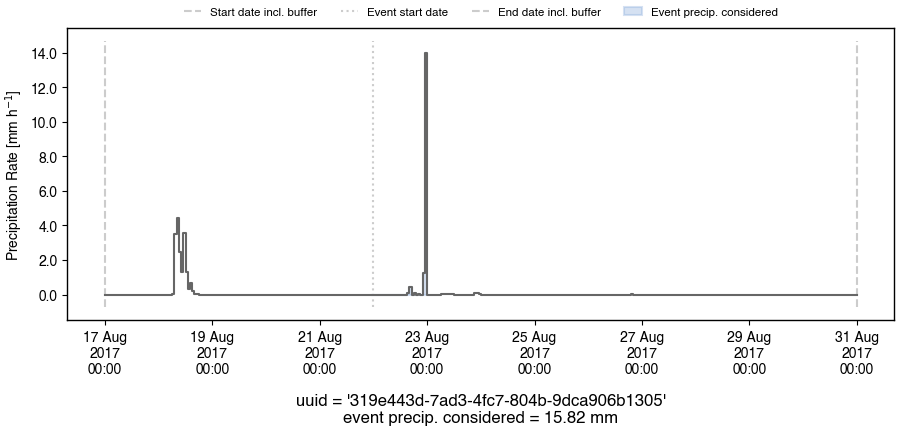
\includegraphics[width=\linewidth]{figures/compare_Geomet_CaSPAr/interpolated_at_stations_occurrence_1036_identified-timesteps_RDRS_v2.1.png}
		\caption{Flood occurrence analyzed using data from CaSPAr NetCDF data (RDRS\_v2.1; 1hr accumulations)}
	\end{subfigure}
	%\vspace*{0.05\textwidth}
	\par\bigskip\bigskip
	\begin{subfigure}[b]{1.0\textwidth}
		\centering
		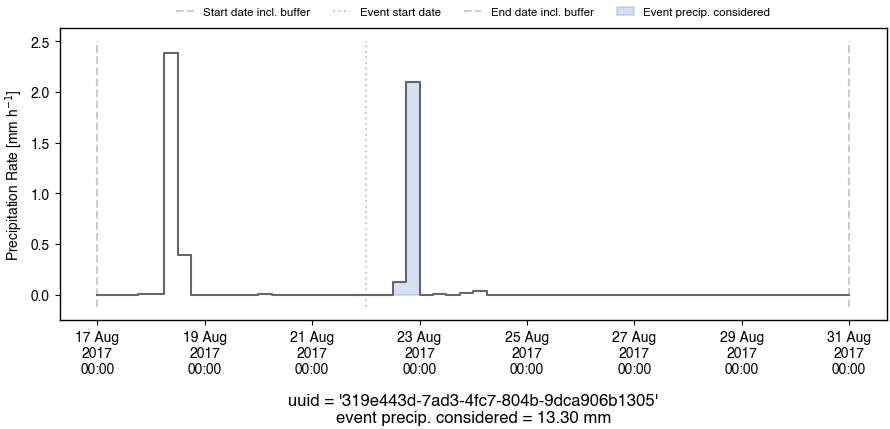
\includegraphics[width=\linewidth]{figures/compare_Geomet_CaSPAr/interpolated_at_stations_occurrence_1036_identified-timesteps_rdpa:10km:6f.png}
		\caption{Flood occurrence analyzed using data from GeoMet GRIB2 data (RDPA; 6hr accumulations)}
	\end{subfigure}
	\par\bigskip\bigskip
	\caption{Flood occurrence in 2017 from HFE database (historical\_flood.json) with UUID ``319e443d-7ad3-4fc7-804b-9dca906b1305''}
\end{figure}
\pagebreak

\begin{figure}[h]
	\begin{subfigure}[a]{1.0\textwidth}
		\centering
		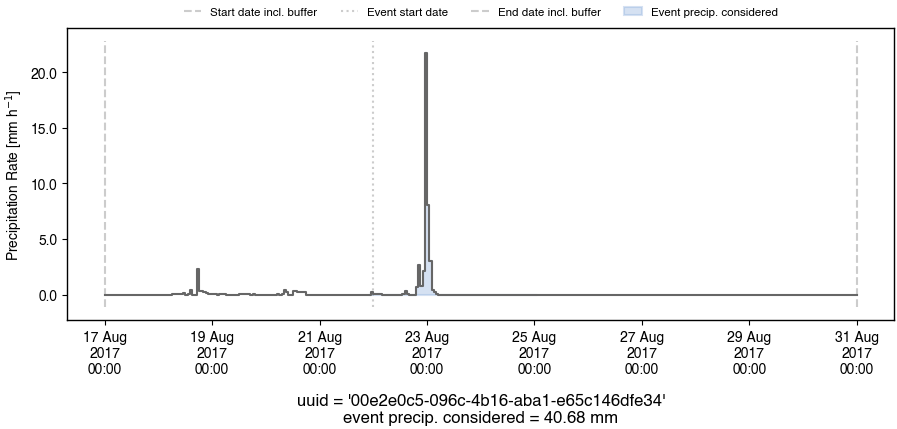
\includegraphics[width=\linewidth]{figures/compare_Geomet_CaSPAr/interpolated_at_stations_occurrence_1043_identified-timesteps_RDRS_v2.1.png}
		\caption{Flood occurrence analyzed using data from CaSPAr NetCDF data (RDRS\_v2.1; 1hr accumulations)}
	\end{subfigure}
	%\vspace*{0.05\textwidth}
	\par\bigskip\bigskip
	\begin{subfigure}[b]{1.0\textwidth}
		\centering
		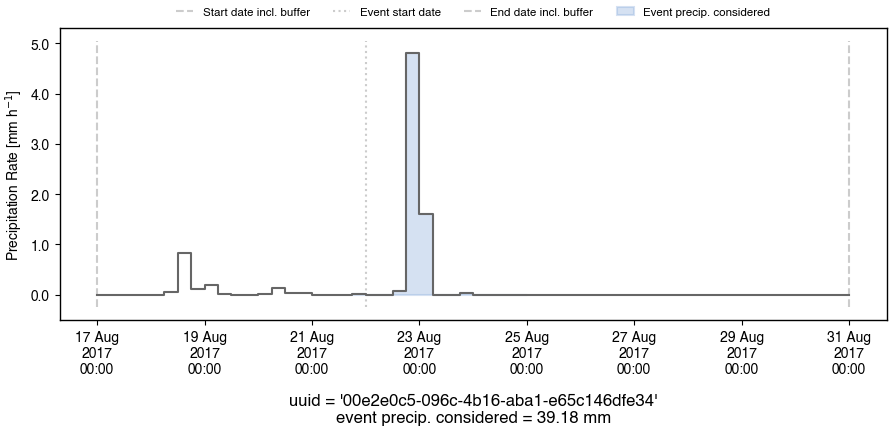
\includegraphics[width=\linewidth]{figures/compare_Geomet_CaSPAr/interpolated_at_stations_occurrence_1043_identified-timesteps_rdpa:10km:6f.png}
		\caption{Flood occurrence analyzed using data from GeoMet GRIB2 data (RDPA; 6hr accumulations)}
	\end{subfigure}
	\par\bigskip\bigskip
	\caption{Flood occurrence in 2017 from HFE database (historical\_flood.json) with UUID ``00e2e0c5-096c-4b16-aba1-e65c146dfe34''}
\end{figure}
\pagebreak

\begin{figure}[h]
	\begin{subfigure}[a]{1.0\textwidth}
		\centering
		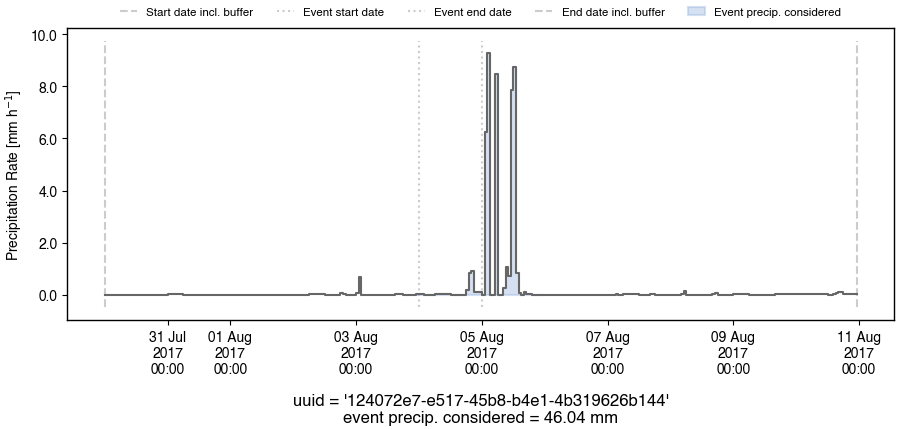
\includegraphics[width=\linewidth]{figures/compare_Geomet_CaSPAr/interpolated_at_stations_occurrence_1054_identified-timesteps_RDRS_v2.1.png}
		\caption{Flood occurrence analyzed using data from CaSPAr NetCDF data (RDRS\_v2.1; 1hr accumulations)}
	\end{subfigure}
	%\vspace*{0.05\textwidth}
	\par\bigskip\bigskip
	\begin{subfigure}[b]{1.0\textwidth}
		\centering
		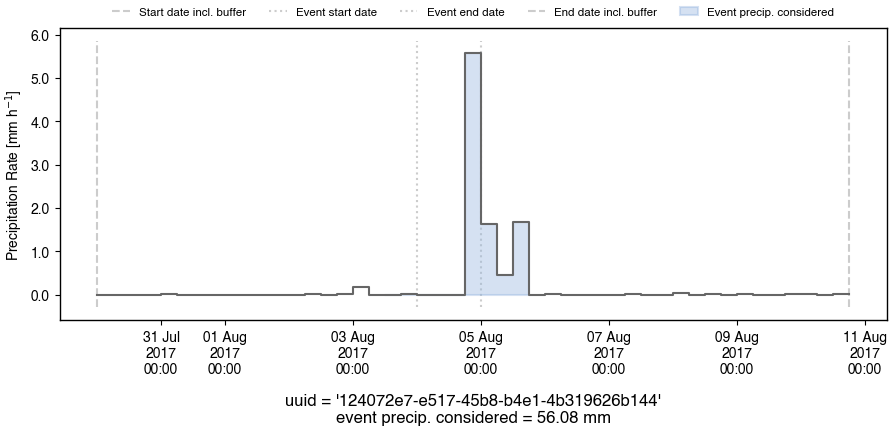
\includegraphics[width=\linewidth]{figures/compare_Geomet_CaSPAr/interpolated_at_stations_occurrence_1054_identified-timesteps_rdpa:10km:6f.png}
		\caption{Flood occurrence analyzed using data from GeoMet GRIB2 data (RDPA; 6hr accumulations)}
	\end{subfigure}
	\par\bigskip\bigskip
	\caption{Flood occurrence in 2017 from HFE database (historical\_flood.json) with UUID ``124072e7-e517-45b8-b4e1-4b319626b144''}
\end{figure}
\pagebreak

\begin{figure}[h]
	\begin{subfigure}[a]{1.0\textwidth}
		\centering
		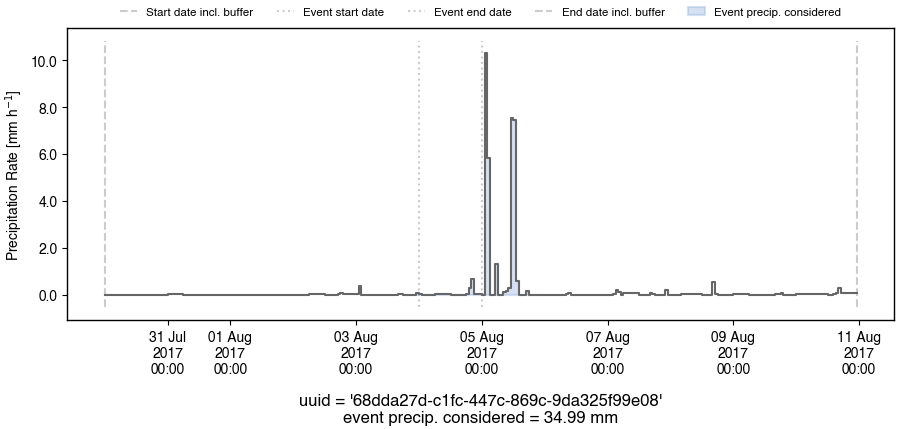
\includegraphics[width=\linewidth]{figures/compare_Geomet_CaSPAr/interpolated_at_stations_occurrence_1057_identified-timesteps_RDRS_v2.1.png}
		\caption{Flood occurrence analyzed using data from CaSPAr NetCDF data (RDRS\_v2.1; 1hr accumulations)}
	\end{subfigure}
	%\vspace*{0.05\textwidth}
	\par\bigskip\bigskip
	\begin{subfigure}[b]{1.0\textwidth}
		\centering
		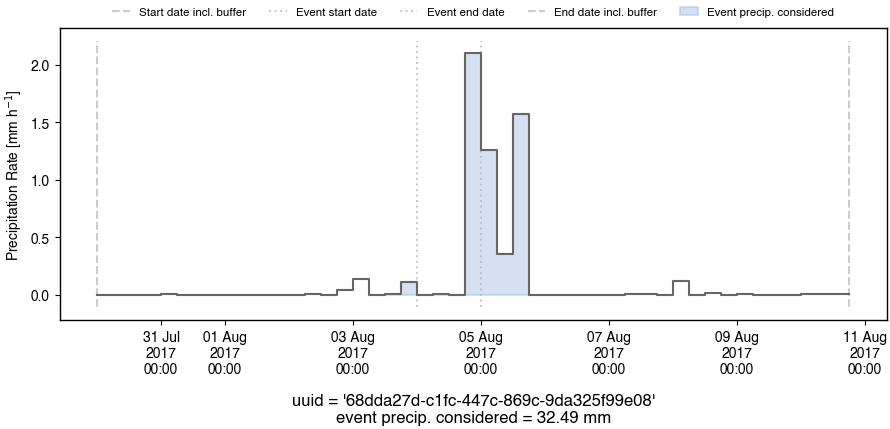
\includegraphics[width=\linewidth]{figures/compare_Geomet_CaSPAr/interpolated_at_stations_occurrence_1057_identified-timesteps_rdpa:10km:6f.png}
		\caption{Flood occurrence analyzed using data from GeoMet GRIB2 data (RDPA; 6hr accumulations)}
	\end{subfigure}
	\par\bigskip\bigskip
	\caption{Flood occurrence in 2017 from HFE database (historical\_flood.json) with UUID ``68dda27d-c1fc-447c-869c-9da325f99e08''}
\end{figure}
\pagebreak

\begin{figure}[h]
	\begin{subfigure}[a]{1.0\textwidth}
		\centering
		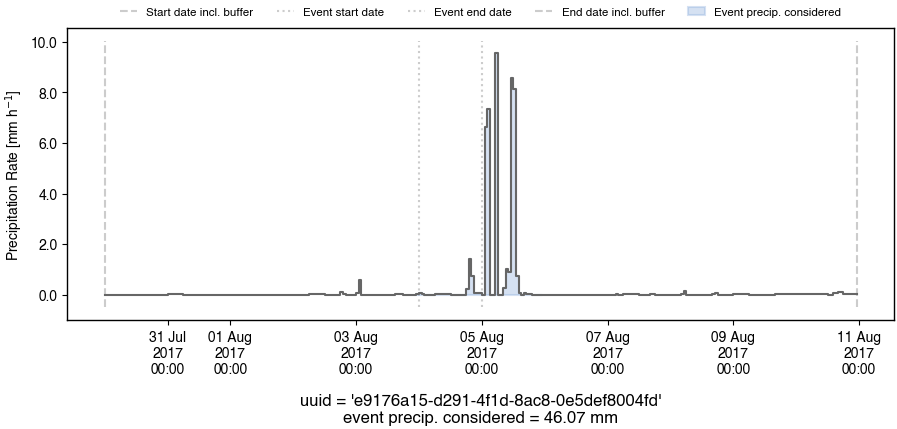
\includegraphics[width=\linewidth]{figures/compare_Geomet_CaSPAr/interpolated_at_stations_occurrence_1058_identified-timesteps_RDRS_v2.1.png}
		\caption{Flood occurrence analyzed using data from CaSPAr NetCDF data (RDRS\_v2.1; 1hr accumulations)}
	\end{subfigure}
	%\vspace*{0.05\textwidth}
	\par\bigskip\bigskip
	\begin{subfigure}[b]{1.0\textwidth}
		\centering
		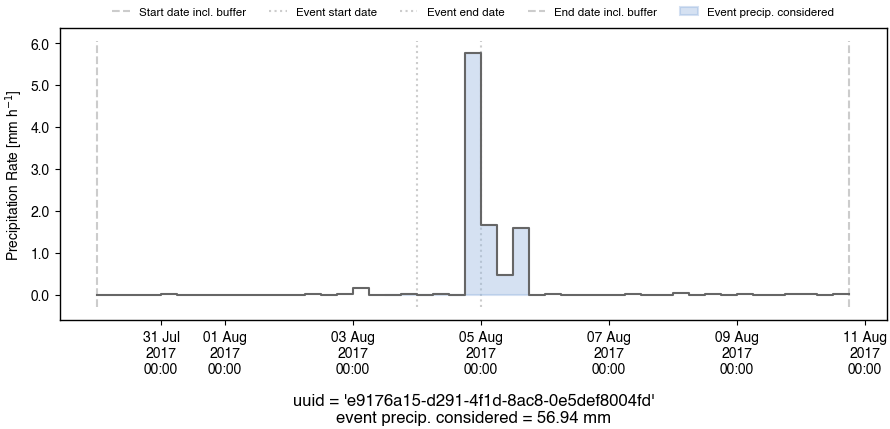
\includegraphics[width=\linewidth]{figures/compare_Geomet_CaSPAr/interpolated_at_stations_occurrence_1058_identified-timesteps_rdpa:10km:6f.png}
		\caption{Flood occurrence analyzed using data from GeoMet GRIB2 data (RDPA; 6hr accumulations)}
	\end{subfigure}
	\par\bigskip\bigskip
	\caption{Flood occurrence in 2017 from HFE database (historical\_flood.json) with UUID ``e9176a15-d291-4f1d-8ac8-0e5def8004fd''}
\end{figure}
\pagebreak

\begin{figure}[h]
	\begin{subfigure}[a]{1.0\textwidth}
		\centering
		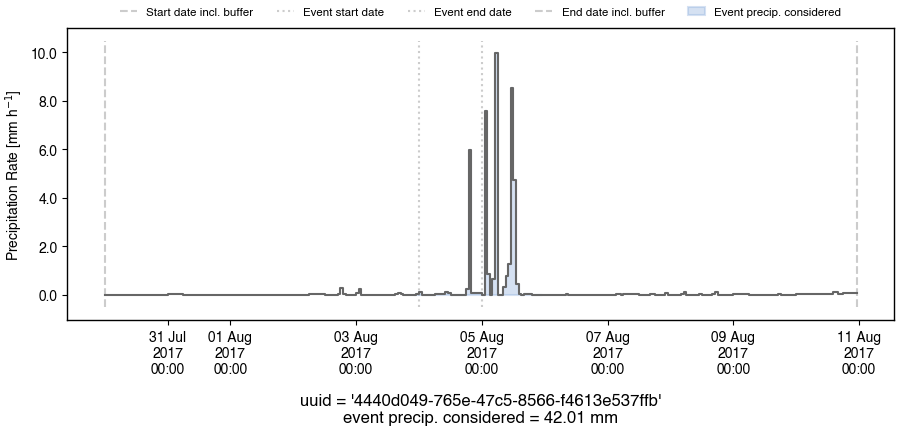
\includegraphics[width=\linewidth]{figures/compare_Geomet_CaSPAr/interpolated_at_stations_occurrence_1059_identified-timesteps_RDRS_v2.1.png}
		\caption{Flood occurrence analyzed using data from CaSPAr NetCDF data (RDRS\_v2.1; 1hr accumulations)}
	\end{subfigure}
	%\vspace*{0.05\textwidth}
	\par\bigskip\bigskip
	\begin{subfigure}[b]{1.0\textwidth}
		\centering
		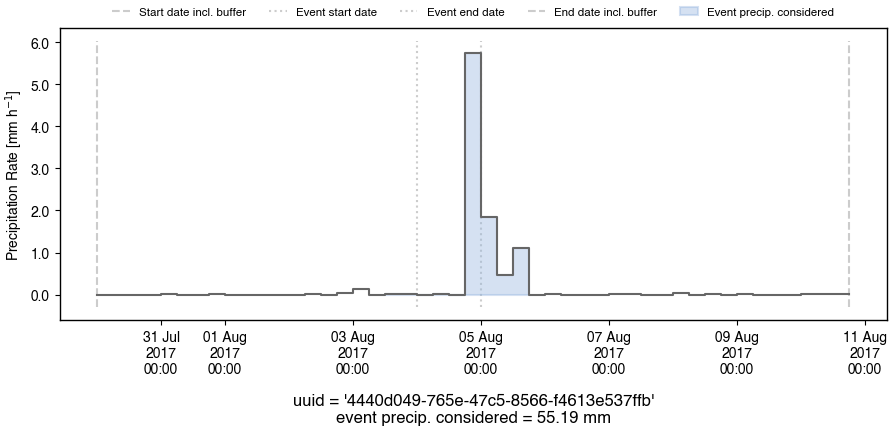
\includegraphics[width=\linewidth]{figures/compare_Geomet_CaSPAr/interpolated_at_stations_occurrence_1059_identified-timesteps_rdpa:10km:6f.png}
		\caption{Flood occurrence analyzed using data from GeoMet GRIB2 data (RDPA; 6hr accumulations)}
	\end{subfigure}
	\par\bigskip\bigskip
	\caption{Flood occurrence in 2017 from HFE database (historical\_flood.json) with UUID ``4440d049-765e-47c5-8566-f4613e537ffb''}
\end{figure}
\pagebreak

\begin{figure}[h]
	\begin{subfigure}[a]{1.0\textwidth}
		\centering
		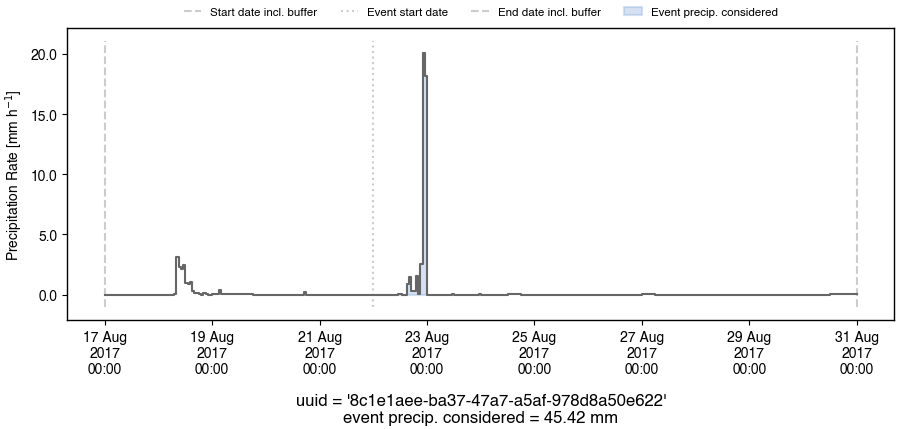
\includegraphics[width=\linewidth]{figures/compare_Geomet_CaSPAr/interpolated_at_stations_occurrence_1157_identified-timesteps_RDRS_v2.1.png}
		\caption{Flood occurrence analyzed using data from CaSPAr NetCDF data (RDRS\_v2.1; 1hr accumulations)}
	\end{subfigure}
	%\vspace*{0.05\textwidth}
	\par\bigskip\bigskip
	\begin{subfigure}[b]{1.0\textwidth}
		\centering
		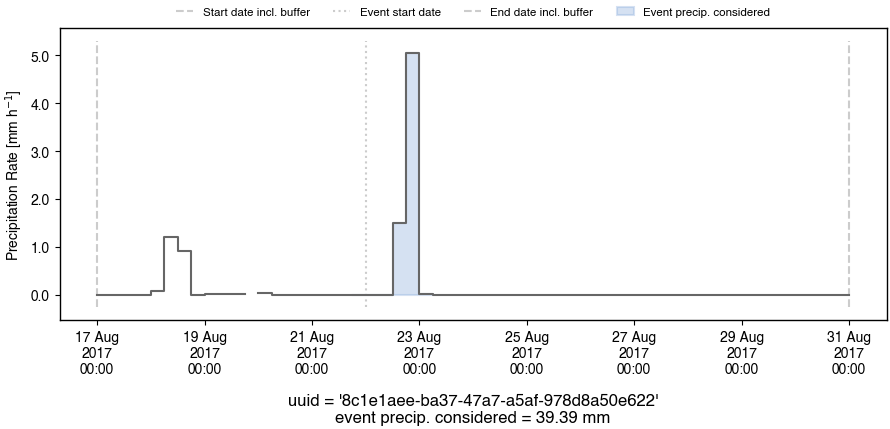
\includegraphics[width=\linewidth]{figures/compare_Geomet_CaSPAr/interpolated_at_stations_occurrence_1157_identified-timesteps_rdpa:10km:6f.png}
		\caption{Flood occurrence analyzed using data from GeoMet GRIB2 data (RDPA; 6hr accumulations)}
	\end{subfigure}
	\par\bigskip\bigskip
	\caption{Flood occurrence in 2017 from HFE database (historical\_flood.json) with UUID ``8c1e1aee-ba37-47a7-a5af-978d8a50e622''}
\end{figure}
\pagebreak

\begin{figure}[h]
	\begin{subfigure}[a]{1.0\textwidth}
		\centering
		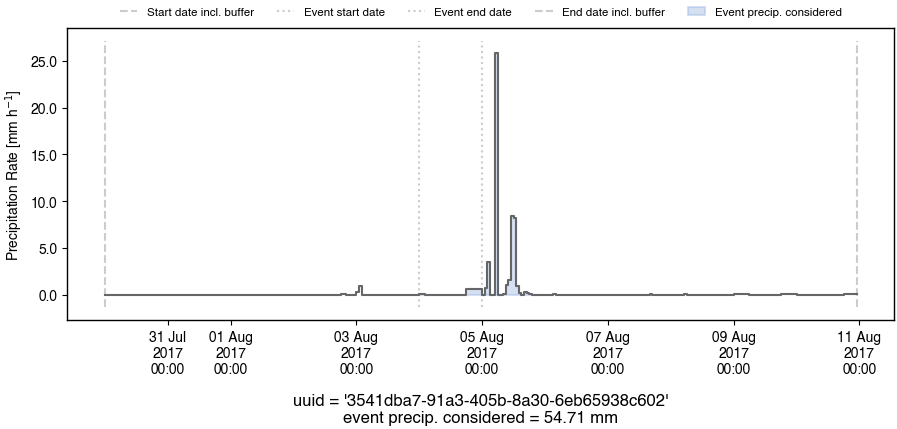
\includegraphics[width=\linewidth]{figures/compare_Geomet_CaSPAr/interpolated_at_stations_occurrence_1303_identified-timesteps_RDRS_v2.1.png}
		\caption{Flood occurrence analyzed using data from CaSPAr NetCDF data (RDRS\_v2.1; 1hr accumulations)}
	\end{subfigure}
	%\vspace*{0.05\textwidth}
	\par\bigskip\bigskip
	\begin{subfigure}[b]{1.0\textwidth}
		\centering
		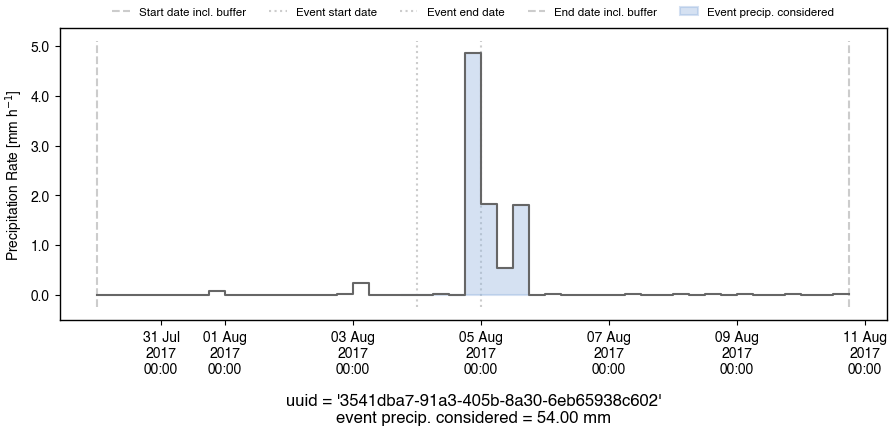
\includegraphics[width=\linewidth]{figures/compare_Geomet_CaSPAr/interpolated_at_stations_occurrence_1303_identified-timesteps_rdpa:10km:6f.png}
		\caption{Flood occurrence analyzed using data from GeoMet GRIB2 data (RDPA; 6hr accumulations)}
	\end{subfigure}
	\par\bigskip\bigskip
	\caption{Flood occurrence in 2017 from HFE database (historical\_flood.json) with UUID ``3541dba7-91a3-405b-8a30-6eb65938c602''}
\end{figure}
\pagebreak

\begin{figure}[h]
	\begin{subfigure}[a]{1.0\textwidth}
		\centering
		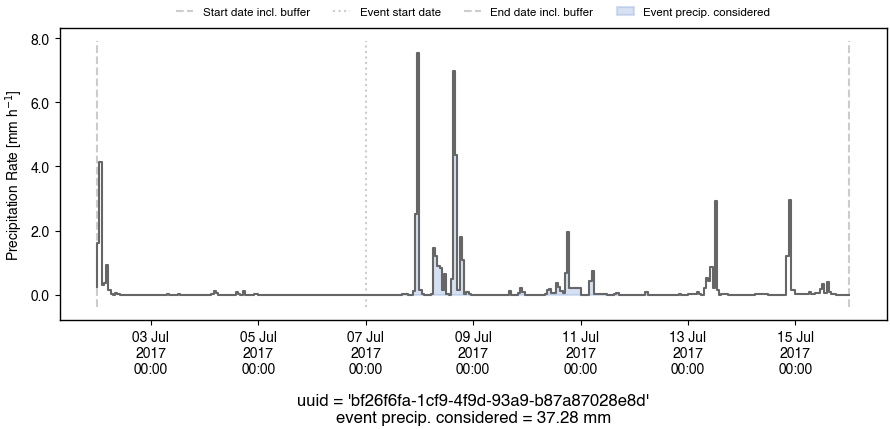
\includegraphics[width=\linewidth]{figures/compare_Geomet_CaSPAr/interpolated_at_stations_occurrence_1362_identified-timesteps_RDRS_v2.1.png}
		\caption{Flood occurrence analyzed using data from CaSPAr NetCDF data (RDRS\_v2.1; 1hr accumulations)}
	\end{subfigure}
	%\vspace*{0.05\textwidth}
	\par\bigskip\bigskip
	\begin{subfigure}[b]{1.0\textwidth}
		\centering
		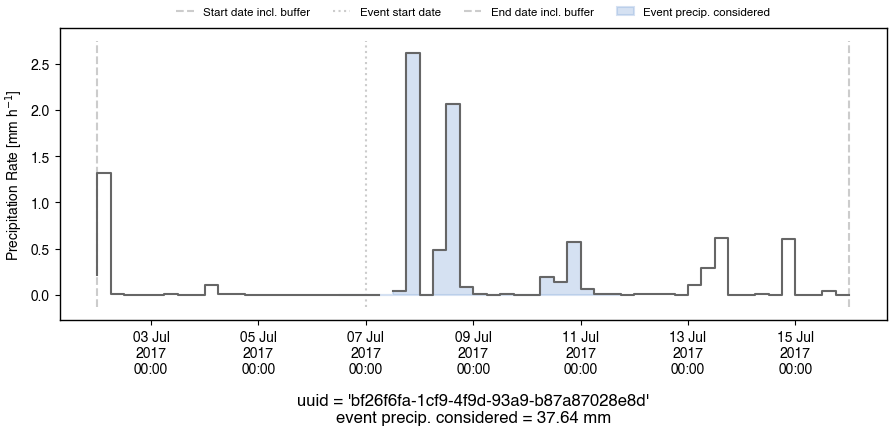
\includegraphics[width=\linewidth]{figures/compare_Geomet_CaSPAr/interpolated_at_stations_occurrence_1362_identified-timesteps_rdpa:10km:6f.png}
		\caption{Flood occurrence analyzed using data from GeoMet GRIB2 data (RDPA; 6hr accumulations)}
	\end{subfigure}
	\par\bigskip\bigskip
	\caption{Flood occurrence in 2017 from HFE database (historical\_flood.json) with UUID ``bf26f6fa-1cf9-4f9d-93a9-b87a87028e8d''}
\end{figure}
\pagebreak

\begin{figure}[h]
	\begin{subfigure}[a]{1.0\textwidth}
		\centering
		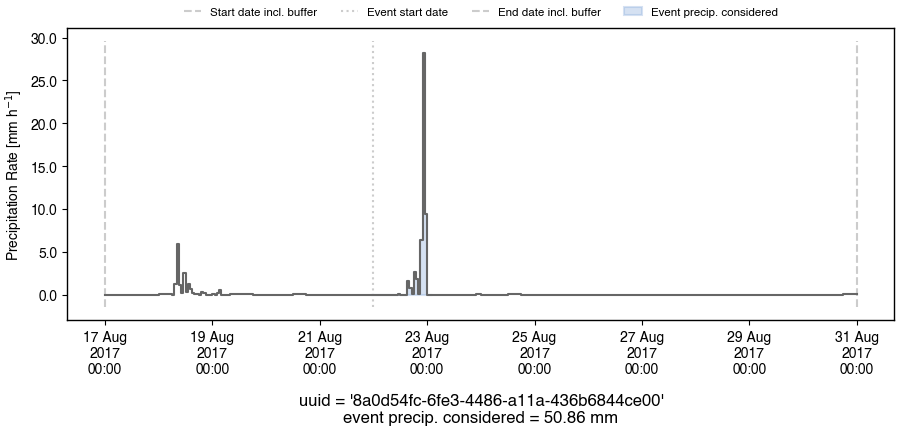
\includegraphics[width=\linewidth]{figures/compare_Geomet_CaSPAr/interpolated_at_stations_occurrence_1464_identified-timesteps_RDRS_v2.1.png}
		\caption{Flood occurrence analyzed using data from CaSPAr NetCDF data (RDRS\_v2.1; 1hr accumulations)}
	\end{subfigure}
	%\vspace*{0.05\textwidth}
	\par\bigskip\bigskip
	\begin{subfigure}[b]{1.0\textwidth}
		\centering
		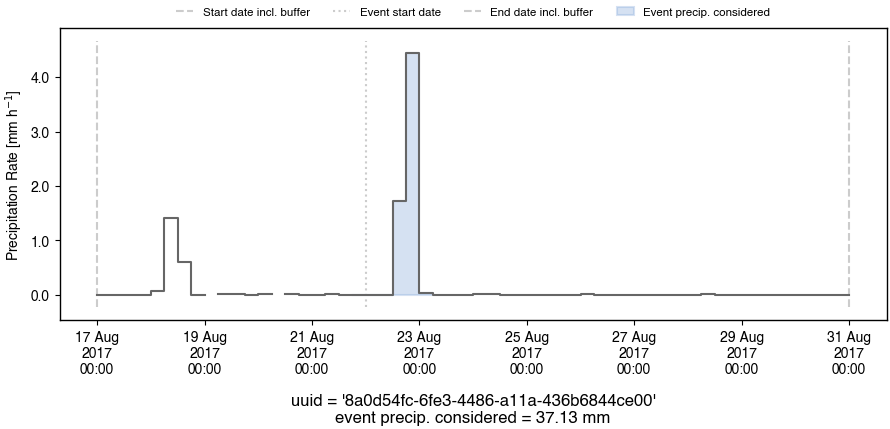
\includegraphics[width=\linewidth]{figures/compare_Geomet_CaSPAr/interpolated_at_stations_occurrence_1464_identified-timesteps_rdpa:10km:6f.png}
		\caption{Flood occurrence analyzed using data from GeoMet GRIB2 data (RDPA; 6hr accumulations)}
	\end{subfigure}
	\par\bigskip\bigskip
	\caption{Flood occurrence in 2017 from HFE database (historical\_flood.json) with UUID ``8a0d54fc-6fe3-4486-a11a-436b6844ce00''}
\end{figure}
\pagebreak

\begin{figure}[h]
	\begin{subfigure}[a]{1.0\textwidth}
		\centering
		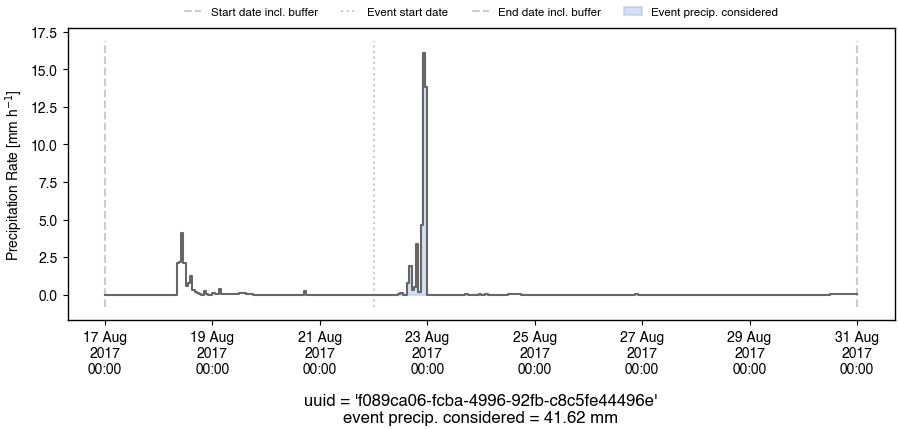
\includegraphics[width=\linewidth]{figures/compare_Geomet_CaSPAr/interpolated_at_stations_occurrence_1478_identified-timesteps_RDRS_v2.1.png}
		\caption{Flood occurrence analyzed using data from CaSPAr NetCDF data (RDRS\_v2.1; 1hr accumulations)}
	\end{subfigure}
	%\vspace*{0.05\textwidth}
	\par\bigskip\bigskip
	\begin{subfigure}[b]{1.0\textwidth}
		\centering
		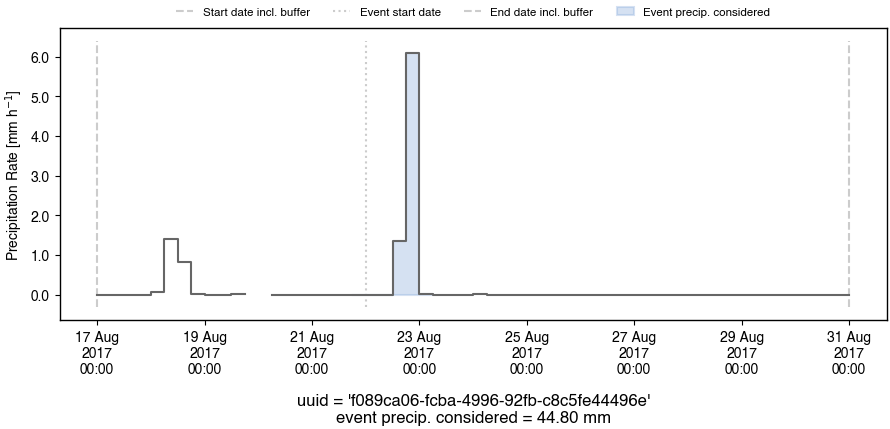
\includegraphics[width=\linewidth]{figures/compare_Geomet_CaSPAr/interpolated_at_stations_occurrence_1478_identified-timesteps_rdpa:10km:6f.png}
		\caption{Flood occurrence analyzed using data from GeoMet GRIB2 data (RDPA; 6hr accumulations)}
	\end{subfigure}
	\par\bigskip\bigskip
	\caption{Flood occurrence in 2017 from HFE database (historical\_flood.json) with UUID ``f089ca06-fcba-4996-92fb-c8c5fe44496e''}
\end{figure}
\pagebreak

\begin{figure}[h]
	\begin{subfigure}[a]{1.0\textwidth}
		\centering
		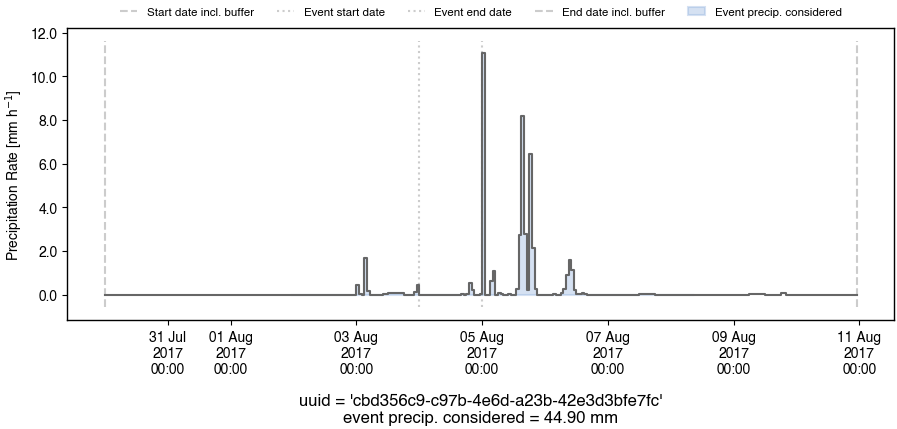
\includegraphics[width=\linewidth]{figures/compare_Geomet_CaSPAr/interpolated_at_stations_occurrence_1534_identified-timesteps_RDRS_v2.1.png}
		\caption{Flood occurrence analyzed using data from CaSPAr NetCDF data (RDRS\_v2.1; 1hr accumulations)}
	\end{subfigure}
	%\vspace*{0.05\textwidth}
	\par\bigskip\bigskip
	\begin{subfigure}[b]{1.0\textwidth}
		\centering
		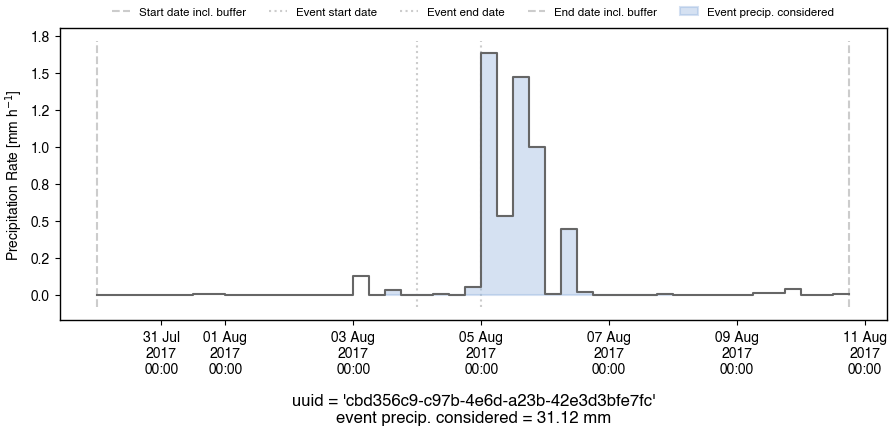
\includegraphics[width=\linewidth]{figures/compare_Geomet_CaSPAr/interpolated_at_stations_occurrence_1534_identified-timesteps_rdpa:10km:6f.png}
		\caption{Flood occurrence analyzed using data from GeoMet GRIB2 data (RDPA; 6hr accumulations)}
	\end{subfigure}
	\par\bigskip\bigskip
	\caption{Flood occurrence in 2017 from HFE database (historical\_flood.json) with UUID ``cbd356c9-c97b-4e6d-a23b-42e3d3bfe7fc''}
\end{figure}
\pagebreak

\begin{figure}[h]
	\begin{subfigure}[a]{1.0\textwidth}
		\centering
		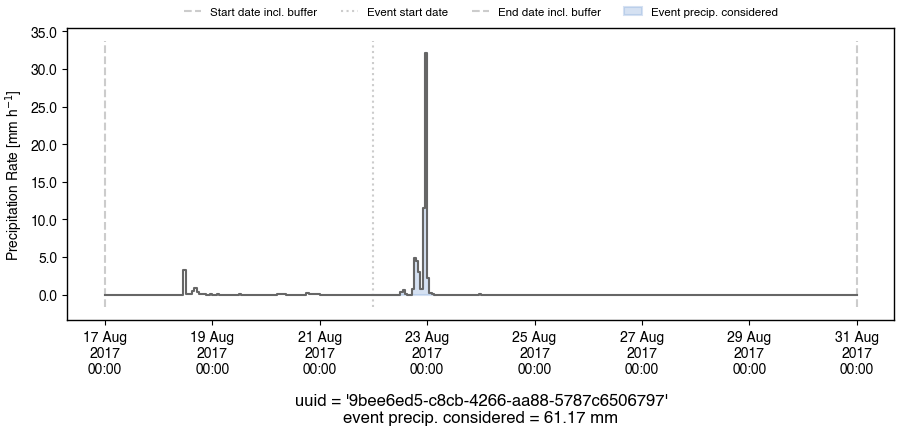
\includegraphics[width=\linewidth]{figures/compare_Geomet_CaSPAr/interpolated_at_stations_occurrence_1686_identified-timesteps_RDRS_v2.1.png}
		\caption{Flood occurrence analyzed using data from CaSPAr NetCDF data (RDRS\_v2.1; 1hr accumulations)}
	\end{subfigure}
	%\vspace*{0.05\textwidth}
	\par\bigskip\bigskip
	\begin{subfigure}[b]{1.0\textwidth}
		\centering
		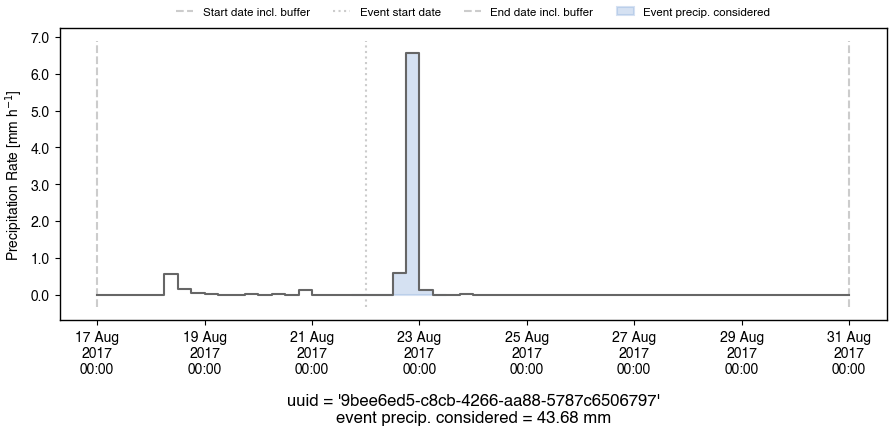
\includegraphics[width=\linewidth]{figures/compare_Geomet_CaSPAr/interpolated_at_stations_occurrence_1686_identified-timesteps_rdpa:10km:6f.png}
		\caption{Flood occurrence analyzed using data from GeoMet GRIB2 data (RDPA; 6hr accumulations)}
	\end{subfigure}
	\par\bigskip\bigskip
	\caption{Flood occurrence in 2017 from HFE database (historical\_flood.json) with UUID ``9bee6ed5-c8cb-4266-aa88-5787c6506797''}
\end{figure}
\pagebreak

\begin{figure}[h]
	\begin{subfigure}[a]{1.0\textwidth}
		\centering
		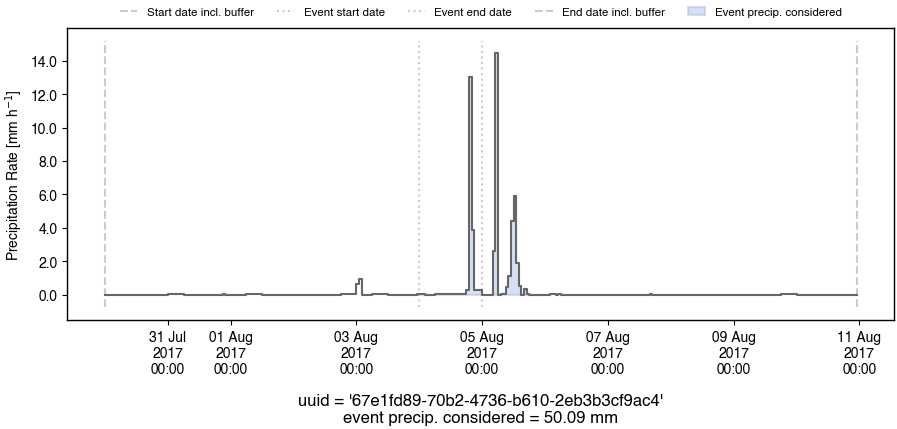
\includegraphics[width=\linewidth]{figures/compare_Geomet_CaSPAr/interpolated_at_stations_occurrence_1737_identified-timesteps_RDRS_v2.1.png}
		\caption{Flood occurrence analyzed using data from CaSPAr NetCDF data (RDRS\_v2.1; 1hr accumulations)}
	\end{subfigure}
	%\vspace*{0.05\textwidth}
	\par\bigskip\bigskip
	\begin{subfigure}[b]{1.0\textwidth}
		\centering
		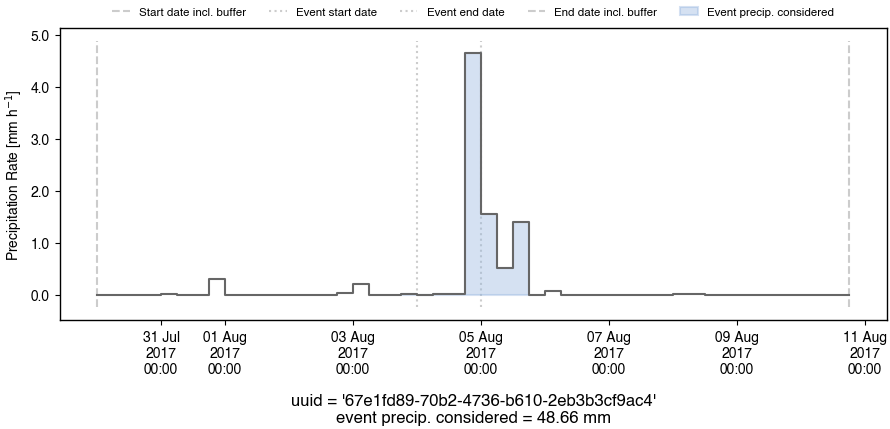
\includegraphics[width=\linewidth]{figures/compare_Geomet_CaSPAr/interpolated_at_stations_occurrence_1737_identified-timesteps_rdpa:10km:6f.png}
		\caption{Flood occurrence analyzed using data from GeoMet GRIB2 data (RDPA; 6hr accumulations)}
	\end{subfigure}
	\par\bigskip\bigskip
	\caption{Flood occurrence in 2017 from HFE database (historical\_flood.json) with UUID ``67e1fd89-70b2-4736-b610-2eb3b3cf9ac4''}
\end{figure}
\pagebreak

\begin{figure}[h]
	\begin{subfigure}[a]{1.0\textwidth}
		\centering
		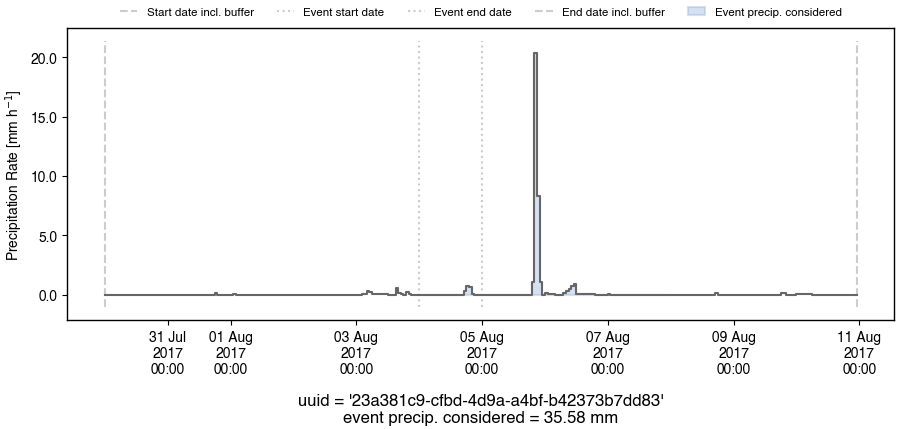
\includegraphics[width=\linewidth]{figures/compare_Geomet_CaSPAr/interpolated_at_stations_occurrence_1756_identified-timesteps_RDRS_v2.1.png}
		\caption{Flood occurrence analyzed using data from CaSPAr NetCDF data (RDRS\_v2.1; 1hr accumulations)}
	\end{subfigure}
	%\vspace*{0.05\textwidth}
	\par\bigskip\bigskip
	\begin{subfigure}[b]{1.0\textwidth}
		\centering
		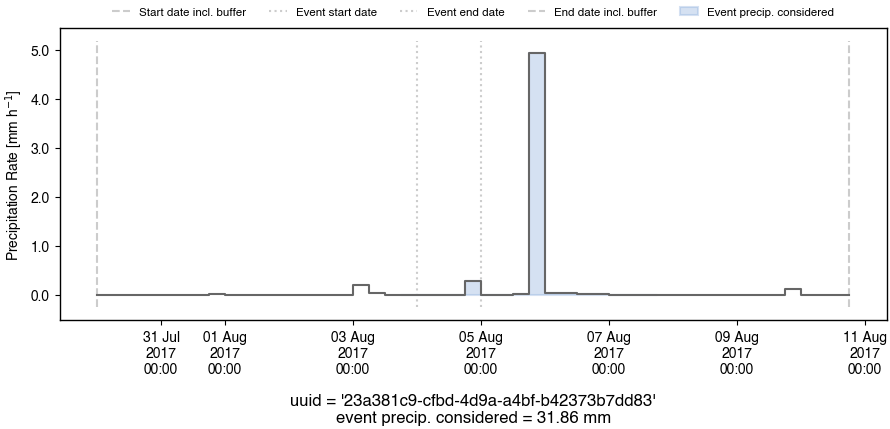
\includegraphics[width=\linewidth]{figures/compare_Geomet_CaSPAr/interpolated_at_stations_occurrence_1756_identified-timesteps_rdpa:10km:6f.png}
		\caption{Flood occurrence analyzed using data from GeoMet GRIB2 data (RDPA; 6hr accumulations)}
	\end{subfigure}
	\par\bigskip\bigskip
	\caption{Flood occurrence in 2017 from HFE database (historical\_flood.json) with UUID ``23a381c9-cfbd-4d9a-a4bf-b42373b7dd83''}
\end{figure}
\pagebreak



\end{document}



